\documentclass[tikz]{standalone}
\usetikzlibrary{positioning}

\begin{document}
	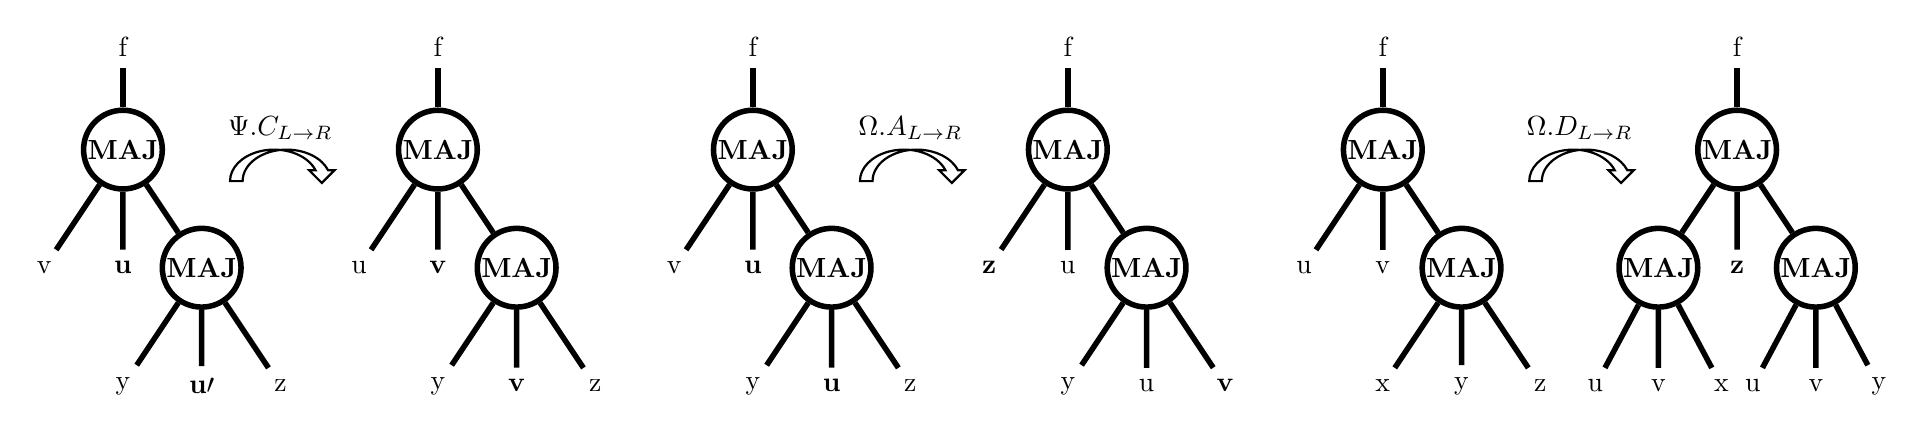
\begin{tikzpicture}[
		line width=2pt,
		level distance=1.5cm,
		sibling distance=1cm,
		maj/.style={ draw, circle, inner sep=0pt, minimum size=1cm, },
		pics/myarrow/.style={
			code={%
				\draw(-6mm,-5mm)arc[start angle=180,delta angle=-160, x radius=7mm, y radius=5mm] -- ++(1mm,0) -- ++(-2mm,-2mm) -- ++(-2mm,2mm) -- ++(1mm,0) arc[start angle=20,delta angle=160, x radius=7mm, y radius=5mm] -- cycle;
				\node[above] at (0,0){#1};
			}
		},
		]
		
		\begin{scope}
			\node[maj](f1){\textbf{MAJ}}
			child{node{v}}
			child{node{\textbf{u}}}
			child{node[maj]{\textbf{MAJ}}
				child{node{y}}
				child{node{\textbf{u$\prime$}}}
				child{node{z}}
			}
			;
			\draw(f1.north)--+(0,.5cm)node[above]{f};
			
			\pic[thick,scale=.8,]at(2cm,0){myarrow={$\Psi.C_{L\rightarrow R}$}};
			
			\node[maj,xshift=4cm](f2){\textbf{MAJ}}
			child{node{u}}
			child{node{\textbf{v}}}
			child{node[maj]{\textbf{MAJ}}
				child{node{y}}
				child{node{\textbf{v}}}
				child{node{z}}
			}
			;
			\draw(f2.north)--+(0,.5cm)node[above]{f};
		\end{scope}
		
		\begin{scope}[xshift=8cm]
			\node[maj](f1){\textbf{MAJ}}
				child{node{v}}
				child{node{\textbf{u}}}
				child{node[maj]{\textbf{MAJ}}
						child{node{y}}
						child{node{\textbf{u}}}
						child{node{z}}
					}
			;
			\draw(f1.north)--+(0,.5cm)node[above]{f};
	
			\pic[thick,scale=.8,]at(2cm,0){myarrow={$\Omega.A_{L\rightarrow R}$}};
			
			\node[maj,xshift=4cm](f2){\textbf{MAJ}}
				child{node{\textbf{z}}}
				child{node{u}}
				child{node[maj]{\textbf{MAJ}}
					child{node{y}}
					child{node{u}}
					child{node{\textbf{v}}}
				}
			;
			\draw(f2.north)--+(0,.5cm)node[above]{f};
		\end{scope}
	
		\begin{scope}[xshift=16cm]
			\node[maj](f1){\textbf{MAJ}}
				child{node{u}}
				child{node{v}}
				child{node[maj]{\textbf{MAJ}}
					child{node{x}}
					child{node{y}}
					child{node{z}}
				}
			;
			\draw(f1.north)--+(0,.5cm)node[above]{f};
			
			\pic[thick,scale=.8,]at(2.5cm,0){myarrow={$\Omega.D_{L\rightarrow R}$}};
			
			\scoped[level 2/.style={sibling distance=.8cm}]
			 \node[maj,xshift=4.5cm](f2){\textbf{MAJ}}
				child{node[maj]{\textbf{MAJ}}
					child{node{u}}
					child{node{v}}
					child{node{x}}
				}
				child{node{\textbf{z}}}
				child{node[maj]{\textbf{MAJ}}
					child{node{u}}
					child{node{v}}
					child{node{y}}
				}
			;
			\draw(f2.north)--+(0,.5cm)node[above]{f};
		\end{scope}
	\end{tikzpicture}
\end{document}